\documentclass[a4paper]{article}
\usepackage{amsfonts}
\usepackage{graphicx}
\usepackage{amsmath}
\usepackage{amssymb}  
\usepackage{cancel}

\begin{document}

\newcommand{\intl}{\displaystyle\int\limits}
  
\noindent \large Auteur: Torben Petré \\
\noindent \large Studierichting: Informatica\\
\noindent \large Oefeningenreeks 5G nr. 1.11\\

\medskip

\normalsize

Bereken het volume $V$ dat men bekomt door de volgende functies op het gegeven interval om de $X$-as te wentelen. Maak telkens een tekening: \\

$f(x)=\tan x$ over interval $\left[0, \dfrac{\pi}{4}\right]$\\

$V = \pi \intl^{\tfrac{\pi}{4}}_0 [ f(x) ]^2dx$ \\

$V = \pi \intl^{\tfrac{\pi}{4}}_0 \tan^2xdx$ \\

$V = \pi \intl^{\tfrac{\pi}{4}}_0 \dfrac{1}{\cos^2x}-1dx$ \\

$V = \pi \left[ \intl^{\tfrac{\pi}{4}}_0 \dfrac{1}{\cos^2x}dx - \intl^{\tfrac{\pi} {4}}_0 dx \right]$ \\

$V = \pi [\tan x-x]^{\tfrac{\pi}{4}}_0$ \\

$V = \pi \left[\tan \dfrac{\pi}{4} - \dfrac{\pi}{4} \right]$ \\

$V = \pi - \dfrac{\pi^2}{4}$ \\

\begin{figure}[h]
\centering  
Afbeelding van de figuur: \\
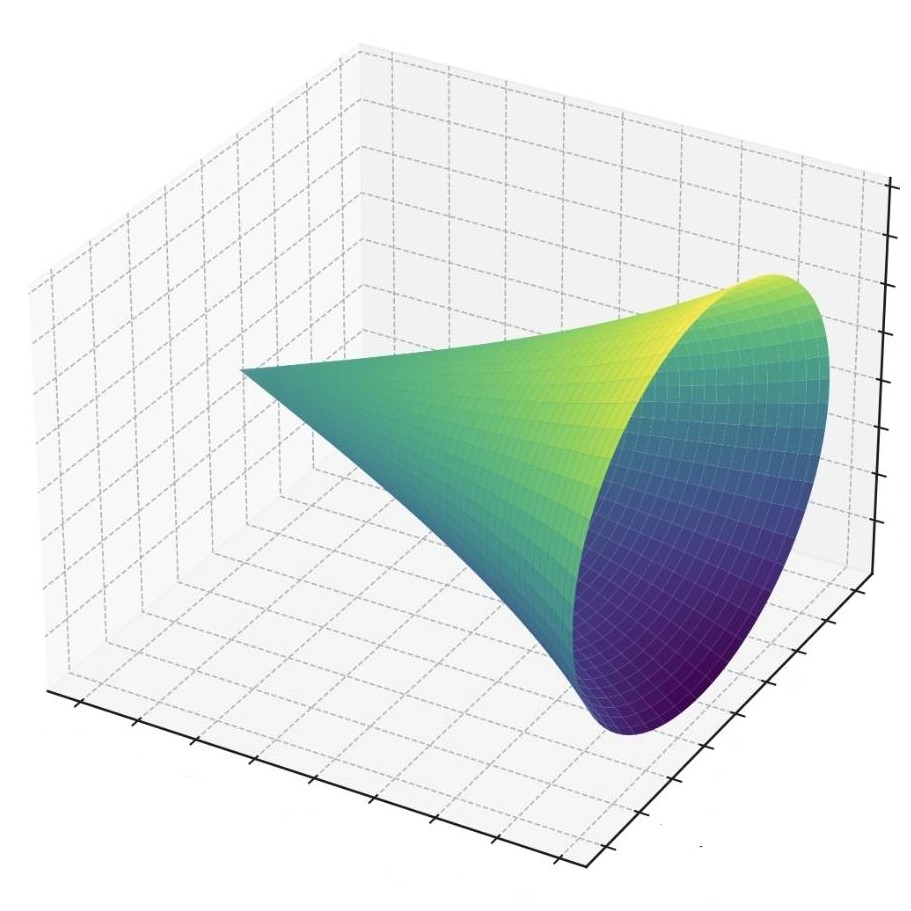
\includegraphics[width=10cm]{5G-1.11-torben.petre.INF.jpg}
\end{figure}

\begin{thebibliography}{999}
%\bibitem{a} Referentie
\end{thebibliography}
\end{document} 